To evaluate the optimization result, we experiment the implementation in a 64 bit Arch Linux machine with Intel CPU of Skylake i7-6600U CPU @ 3GHz. The compiler and arithmetic environment are as following: 

  \begin{itemize}
  \setlength\itemsep{0.5em}
  \item{GCC 6.1.1 compiler}
  \item{64 bit multiplication (mul, mulx): 1 op/cycle}
  \item{64 bit addition/subtraction (add, sub): 4 op/cycle}
  \item{64 bit addition with carry (adc, adcx, adox): 1 op/cycle}
  \item{Carry addition only: peak performance of 2 ops/cycle ~6 Gops/s on 1 core}
  \item{Compile flag: -O3 -mavx2 -mbmi2 -madx}
  \end{itemize}
  \setlength\itemsep{1.5em}
Based on the recommended Elliptic curve parameters from the guidance standard \cite{Brown:2010}, we have chosen five predefined curves with various key sizes: 192, 224, 256, 384, 521 bits. All versions of implementation have been validated by using Google Unit test, by checking the ECDH key exchange result. The benchmark is done by calculating the CPU cycles, in order to testify the real performance by eliminating the influence of the machine. In the end we compare our implementation with OpenSSL, the well known open source library to check our implementation effect. The library has been compiled locally and used as headers. 

\begin{figure}[h!]\centering
  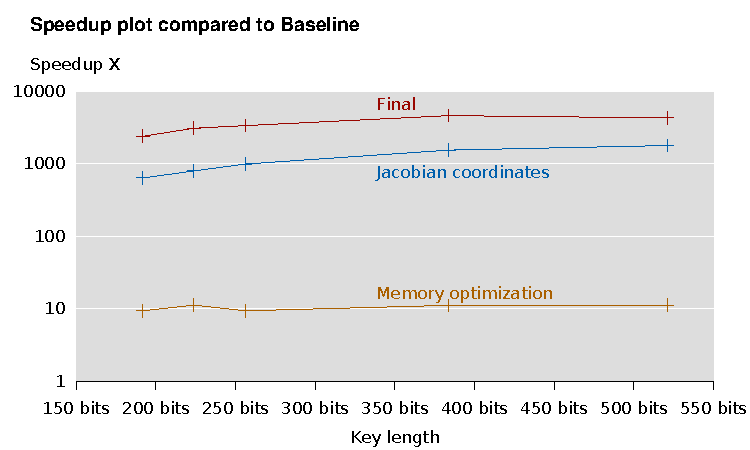
\includegraphics[scale=0.7]{speedup}
  \caption{Speedup plot compared to Baseline \label{speedup}}
\end{figure}
\begin{figure}[h!]\centering
  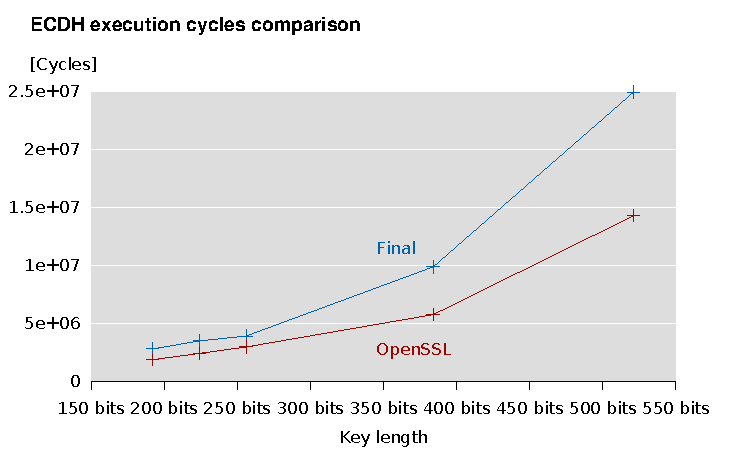
\includegraphics[scale=0.7]{ecdh}
  \caption{ECDH execution cycles comparison\label{ecdh}}
\end{figure}
\begin{figure}[h!]\centering
  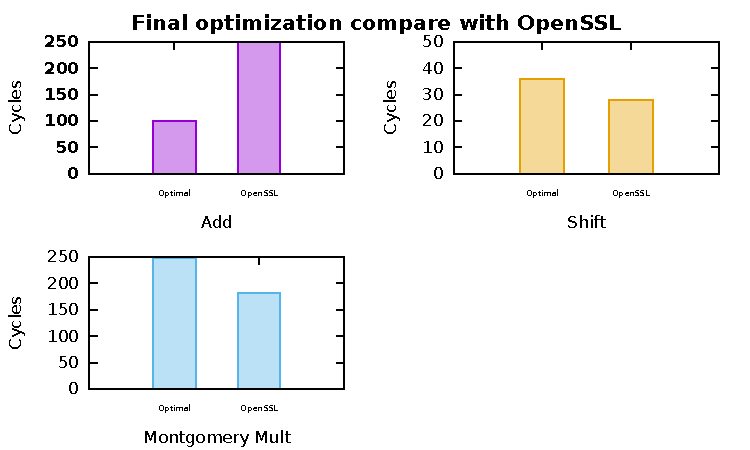
\includegraphics[scale=0.7]{openssl}
  \caption{Final optimization compared with OpenSSL\label{openssl}}
\end{figure}

In the speedup comparison(Fig.~\ref{speedup}) three crucial numbers are shown. It can be clearly seen that the Final implementation can execute the key exchange process 5000 times(TO BE CHANGED) faster than the baseline in almost all the key lengths. In all three cases the speedup increases as the key size grows. It can be explained that this version of code is not fully running through its potential with relatively shorter the key size, considering that the big integer operations(64 bits base) will go through a complete operations even with smaller input size. The first milestone of memory optimization gives us about 10 times speedup, whereas Jacobian coordinates version of code can run 1000 times(TO BE CHANGED) faster. This is due to the fact that the algorithm thus the operation count has changed fundamentally after we apply the projective coordinates and precomputed the Elliptic curve points in order to save unnecessary operations. The speedup result is satisfactory and reasonable as the first two versions of implementations contain costly memory allocations and expensive computation that can be avoided. The real performance boost is between the Final version and Jacobian coordinates, after applying the CPU based optimizations mentioned in previous section 3. It can be seen that it give us another 5x(TO BE CHANGED) speedup, showing the efficiency of the final implementation.



Next we run the same operation with OpenSSL library and compare their computation cycles with us. It is no surprise that with the increasing of the key length the required cycles also increase rapidly(Fig.~\ref{ecdh}). Our number of required cycles remains the save level with OpenSSL, in key length range of less than 256 bits, yet falls behind OpenSSL with larger key length. 



Individual operations of integers are the main component of our algorithm. To see how good is our implementation we choose integer addition, shift and Montgomery multiplication to compare with OpenSSL(Fig.~\ref{openssl}).This comparison is done with the same random large integers for both Final implementation and OpenSSL. In the comparison of integer addition, our final implementation uses less cycles than OpenSSL's big integer addition thus being faster than OpenSSL. Yet in both shift and Montgomery multiplication our implementation is more expensive thus runs slower than OpenSSL. 

\begin{figure}[h!]\centering
  \includegraphics[scale=0.7]{perfplot1}
  \caption{Performance plot of baseline and memory optimization\label{perfplot1}}
\end{figure}
\begin{figure}[h!]\centering
  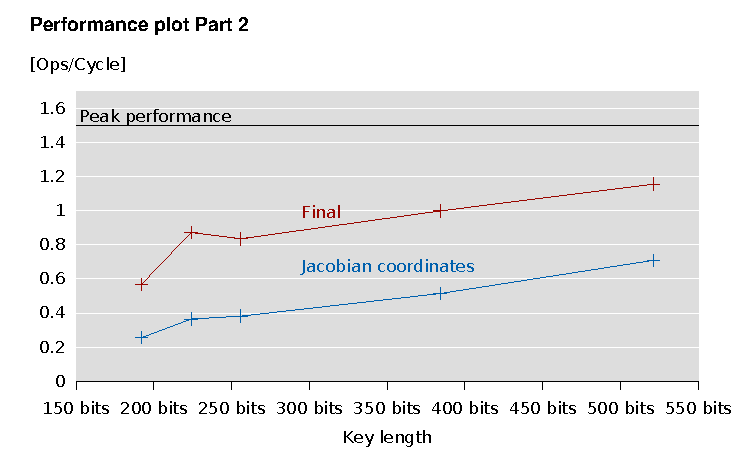
\includegraphics[scale=0.7]{perfplot2}
  \caption{Performance plot of Final optimization and Jacobian coordinates\label{perfplot2}}
\end{figure}

Performance plots(Fig.~\ref{perfplot1} and Fig.~\ref{perfplot2}) are consisted with the division of operation counts and cycles. It reflects if the implementation can make the best use of the machines' computation ability. Normally in order to show the real performance improvement, operation count would stay constant as the optimization goes on. Yet in our case since the integer operations does not only include the computational integer operations, but also include the index counts operations that are generated during looping. Thus we have to compromise by using code generated operation counts. In the following performance plots the operation counts varies, but it does reflect the computational efficiency of the code in certain level. In Fig.~\ref{perfplot1} the first comparison is done by showing the effect of memory optimization. It is clear that with large amount of memory allocation, the baseline performance is really limited. In Fig.~\ref{perfplot2} we begin to see the real performance boost that comes from later optimization. Between these two figures the operation counts change drastically, thus we separate the performance plots. The peak performance here is calculated by considering the ratio of additions and multiplications. With 1 add and 1 mult per cycle and two times of add out of one mult (2 add : 1 mult), we can draw the line of peak performance at 1.5 ops/cycle. As we can see the final optimization are close to the peak performance with large key size. The highest performance of the final implementation arrives when the key length of 521 bits, with 1.15/1.5 = 77\% of the peak performance.
\begin{figure}[h!]\centering
  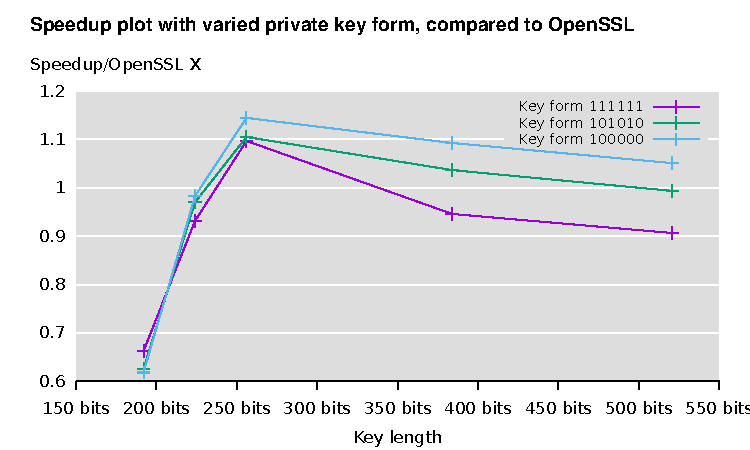
\includegraphics[scale=0.7]{keysize}
  \caption{Speedup plot with varied private key form, compared to OpenSSL\label{keysize}}
\end{figure}

Fig.~\ref{keysize} gives us another perspective of how different key forms could influence the speedup.  In all the simplified private key form that consist of only zeros and ones, our speed of processing EDCH is faster than OpenSSL. The key forms that consist only ones has the worst performance since it requires redundant integer operations that are unavoidable. It is an interesting future work that would allow us to optimize the algorithm based on the combinations of varied key forms. 